\documentclass[12pt,a4paper,titlepage,twoside]{report}
\usepackage[T1]{fontenc}
\usepackage[english, spanish, catalan]{babel}
\usepackage[utf8x]{inputenc}
\usepackage[gen]{eurosym}	%Inclou el simbol del euro
\usepackage{lmodern}
\usepackage{xcolor}
\usepackage{import}
\usepackage{svg}
\usepackage{fancyhdr}
\usepackage{listings} %FOR CODE HIGHLIGHTING!
\usepackage[numbers]{natbib}
%\usepackage{lscape}	%Permet inserir pagines orientades en landscape (no es gira en pantalla per una millor lectura
\usepackage{pdflscape} %Permet inserir pagines orientades en landscape (es gira en pantalla)

% Permet inserir PDFs com a part del document
\usepackage{pdfpages}

%Permet posar imatges de backgrounds, per exemple per portades de treballs
\usepackage{eso-pic}

\usepackage{mdframed} %Permet tancar text en un requadre, inclus text tabulat amb tabbing o tabular que normalment falla.

%Paquet de matemàtiques per poder tenir més opcions a l'hora de fer fòrmules
\usepackage{mathtools}
\usepackage{amsmath}

%Redeclaració de la funció valor absolut per a les formules \[ \abs*{...} \]
\DeclarePairedDelimiter\abs{\lvert}{\rvert}

%Per tal que la bibliografia surti a la taula de continguts
%\usepackage[nottoc, numbib]{tocbibind}

%Per poder posar hipervincles en el document
\usepackage[colorlinks=true, pagebackref=false, citecolor=blue, urlcolor=blue, citecolor=blue, linktoc=page, linkbordercolor={0.7 0.7 1}, citebordercolor={0.7 0.7 1}, urlbordercolor={0.7 0.7 1}]{hyperref}

%Compressió d'imatges per a pdfLatex
%\pdfminorversion=5 
%\pdfcompresslevel=9
%\pdfobjcompresslevel=2

% Paquet per a efectuar comentaris
\usepackage{verbatim}

% Permet prevenir que es trenquin paraules a final de linia i que les divideixi amb el format angles
\usepackage[none]{hyphenat}

% Paquet per a importar imatges i path relatiu a aquest main on les va a buscar
\usepackage{graphicx}
\graphicspath{{./img/}}

% Marges i espaiats
\usepackage[top=2cm,left=2cm,right=2cm,bottom=2cm]{geometry}
\usepackage{enumitem}
\usepackage{varwidth}% http://ctan.org/pkg/varwidth   	(Centrat pero dins del centrat	que estigui aliniat a l'esquerra)

%Format de les figures
\usepackage{chngcntr}
\usepackage{float}
\counterwithout*{figure}{section}

% Taula de continguts
\usepackage{titletoc}% http://ctan.org/pkg/titletoc
\usepackage[nottoc]{tocbibind} %Fa que surti la bibliografia a la TOC

% Format per a la taula de continguts (Index)
\titlecontents*{chapter}% <section-type>
  [0pt]% <left>
  {\addvspace{1em}}% <above-code>
  {\bfseries\chaptername\ \thecontentslabel\quad}% <numbered-entry-format>
  {}% <numberless-entry-format>
  {\bfseries\hfill\contentspage}% <filler-page-format>

% Evita l'overlapping de la taula de continguts quan té apartats buits
\usepackage{tocloft}
\setlength{\cftpartnumwidth}{4em} % change the width of the part number
\begin{comment}
\makeatletter
\renewcommand{\l@chapter}{\@dottedtocline{1}{1.5em}{2.6em}}
\renewcommand{\l@subsection}{\@dottedtocline{2}{3.8em}{3.2em}}
\renewcommand{\l@subsubsection}{\@dottedtocline{3}{7.0em}{4.1em}}
\renewcommand{\l@paragraph}{\@dottedtocline{4}{10em}{5em}}
\renewcommand{\l@subparagraph}{\@dottedtocline{5}{12em}{6em}}
\renewcommand{\l@figure}{\@dottedtocline{1}{1.5em}{2.3em}}
\let\l@table\l@figure
\makeatother
\end{comment}

%Inicialització de l'estil de la pàgina
\pagestyle{fancy}
\fancyhf{}
\fancyhead[LE,RO]{\nouppercase \rightmark}
\fancyhead[LO,RE]{\nouppercase \leftmark}
\fancyfoot[C]{\thepage}

\newcommand{\Keywords}[1]{\vfill\noindent{\small{\em Paraules clau}: #1}}
\definecolor{grisclar}{gray}{0.5}
\definecolor{grisfosc}{gray}{0.25}

% ############# Redefinició de comandes existents
% Fa que els itemizes no tinguin espaiat entre els items
\newenvironment{sitemize}{ %Short Itemize
  \begin{itemize}
  \setlength{\itemsep}{0pt}
  \setlength{\parskip}{0pt}
  \setlength{\parsep}{0pt}
}{
  \end{itemize}
}

% Fa que els enumerate no tinguin espaiat entre els items
\newenvironment{senumerate}{ %Short Enumerate
  \begin{enumerate}
  \setlength{\itemsep}{0pt}
  \setlength{\parskip}{0pt}
  \setlength{\parsep}{0pt}
}{
  \end{enumerate}
}

% Editar con los datos correspondientes
\newcommand{\titulo}{Desenvolupament d'un motor per jocs de rol 2.5D per Nintendo Switch i PC}
\newcommand{\titulacion}{Grau en Enginyeria Informàtica. Pla 2015}
\newcommand{\doc}{Memòria}
\newcommand{\autor}{Lluís Trilla i Esquinas}
\newcommand{\director}{Dr. Gustavo Patow}
\newcommand{\departament}{Informàtica, Matemàtica Aplicada i Estadística}
\newcommand{\deparea}{LSI}
\newcommand{\convocatoria}{9/2020}

% Tags nous especials per projectes Gus ; )
\newcommand{\bE}{\textnormal{\textbf{building}Engine}}
\newcommand{\sE}{\textnormal{\textbf{skyline}Engine}}

% START APPENDIX FUNCTIONALITIES
\renewcommand\appendix{\par
  \setcounter{chapter}{0}%
  \setcounter{section}{0}%
  \gdef\@chapapp{\appendixname}%
}

\usepackage{appendix}
\renewcommand{\appendixtocname}{Llista d'annexos}
% END APPENDIX FUNCTIONALITIES

\title{\titulo}
\author{\autor}

% ELS CAPÍTOLS HAN D'ANAR EN UNA SUBCARPETA ANOMENADA '/capitols/' 
% EN UNA SUBCARPETA RELATIVA A LA LOCALITZACIÓ D'AQUEST FITXER 

\begin{document}
\setcounter{secnumdepth}{3}

% #######################################################
% #Template per a PFC/TFM/TFG... by Alejandro Arangua Rovira - 2013 #
% #######################################################

% #################################################################
% - Les imatges han d'anar en una subcarpeta relativa a aquest fitxer anomenada /img/
% #################################################################

\begin{titlepage}
\begin{center}

% Logos UdG
\begin{minipage}{0.49\linewidth}
\begin{flushleft}

\includegraphics[height=1.5cm]{./img/logos/EPS}
\end{flushleft}
\end{minipage}
\begin{minipage}{0.49\linewidth}
\begin{flushright}
%
\includegraphics[height=1.5cm]{./img/logos/imae_logo} %Segon logo de la dreta en cas de necessitar-se
\end{flushright}
\end{minipage}

\vspace{2cm}

\begin{color}{grisfosc}
\large
Escola Politècnica Superior\\[0.2cm]
Universitat de Girona\\[1.9cm]
\end{color}

{\LARGE \bfseries \titulo}\\[1.5cm]
\textsc{\large Projecte/Treball Fi de Carrera}\\[0.4cm]
\textcolor{grisclar}{\large\titulacion}\\[5.0cm]

%IMATGE PORTADA
\AddToShipoutPicture*{%
\put(68,225){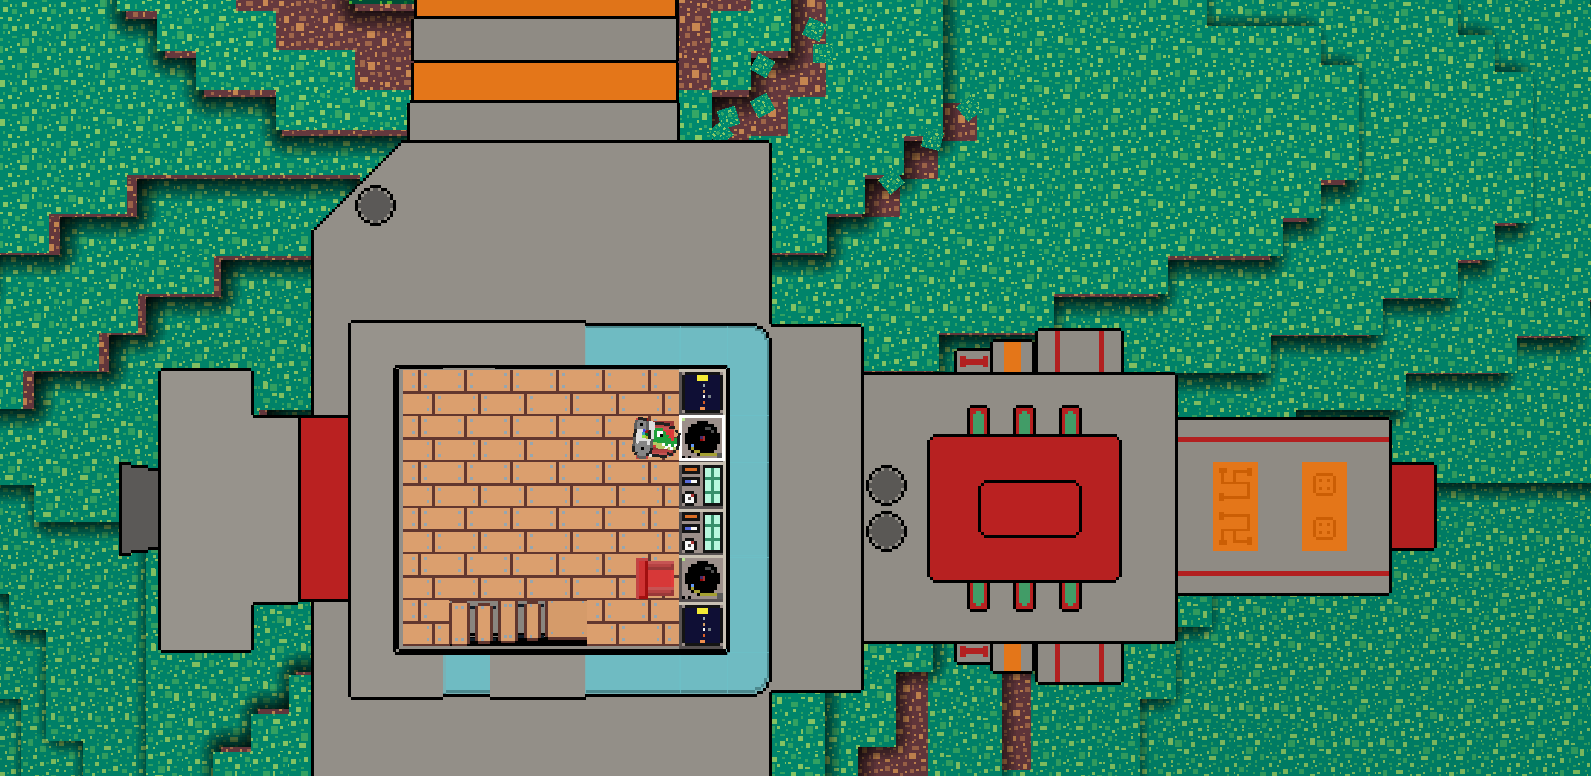
\includegraphics[width=\textwidth]{/novanovaportada.png}}%
}
\vspace{5cm}

% Autor, director y fecha
\begin{flushleft} \large
\emph{Document:} \doc\\[0.15cm]
\emph{Autor:} \autor\\[0.15cm]
\emph{Director:} \director\\[0.15cm]
\emph{Departament:} \departament\\[0.15cm]
\emph{Àrea:} \deparea\\[0.15cm]
\emph{Convocatoria:} \convocatoria\\[0.15cm]
%\today
\end{flushleft}

%\vfill
% Bottom of the page
%{\large \today}

\end{center}

\end{titlepage}


\tableofcontents
\chapter{Introducció}
\label{chap:c1}
	\subimport{capitols/}{Capitol1.tex}
\chapter{Estudi de viabilitat}
\label{chap:c2}
	\subimport{capitols/}{Capitol2.tex}
\chapter{Metodologia}
\label{chap:c3}
	\subimport{capitols/}{Capitol3.tex}
\chapter{Planificació}
\label{chap:c4}
	\subimport{capitols/}{Capitol4.tex}
\chapter{Marc del treball}
\label{chap:c5}
	\subimport{capitols/}{Capitol5.tex}
\chapter{Requisits del sistema}
\label{chap:c6}
	\subimport{capitols/}{Capitol6.tex}
\chapter{Estudis i decisions}
\label{chap:c7}
	\subimport{capitols/}{Capitol7.tex}
\chapter{Anàlisis i disseny}
\label{chap:c8}
	\subimport{capitols/}{Capitol8.tex}
\chapter{Implementació i proves}
\label{chap:c9}
	\subimport{capitols/}{Capitol9.tex}
\chapter{Resultats}
\label{chap:c10}
	\subimport{capitols/}{Capitol10.tex}
\chapter{Conclusions}
\label{chap:c11}
	\subimport{capitols/}{Capitol11.tex}
\chapter{Treball Futur}
\label{chap:c12}
	\subimport{capitols/}{Capitol12.tex}

\nocite{*}

\bibliographystyle{plainnat}
\bibliography{bibliografia}
\pagebreak
%\subimport{capitols/}{Annex.tex}

\chapter{Manual d'usuari}
\label{chap:manual}
	\subimport{capitols/}{manual.tex}
\end{document}
